\documentclass[journal]{IEEEtran}
\usepackage{cite}
\usepackage{amsmath,amssymb}
\usepackage{graphicx}
\usepackage{booktabs}
\usepackage{array}
\usepackage{algorithm}
\usepackage{algorithmic}
\usepackage{url}
\usepackage{orcidlink}
\usepackage{xcolor}
\graphicspath{{Figures/}}
\newcommand{\Pbb}{\mathbb{P}}
\newcommand{\Ebb}{\mathbb{E}}

\begin{document}
\title{Site-Calibrated and Auditable Zero-Trust Intrusion Detection for Industrial IoT: A Leakage-Audited Study}

\author{Ali~Akhmetkaliyev \orcidlink{0009-0002-6689-9066}, Mohammed~Alaa~Ala'anzy,~\IEEEmembership{Senior~Member,~IEEE} \orcidlink{0000-0002-0005-7037}, and Yassine Himeur,~\IEEEmembership{Senior~Member,~IEEE} \orcidlink{0000-0001-8904-5587}
\thanks{Ali Akhmetkaliyev is with Department of Information Systems, SDU University, Kaskelen~040900, Kazakhstan (e-mail: 251107004@sdu.edu.kz).}
\thanks{Mohammed Alaa Ala'anzy is with Department of Computer Science, SDU University, Kaskelen~040900, Kazakhstan (e-mail: m.alanzy@ieee.org).}
\thanks{Yassine Himeur is with College of Engineering and Information Technology, University of Dubai, Dubai, United Arab Emirates (e-mail: yhimeur@ud.ac.ae).}
\thanks{(Corresponding author: Mohammed Alaa Ala'anzy.)}}

\markboth{Manuscript under review}{Akhmetkaliyev \MakeLowercase{\textit{et al.}}: Site-Calibrated Zero-Trust Intrusion Detection for Industrial IoT}
\maketitle

\begin{abstract}
High reported accuracies for Industrial IoT intrusion detection can reflect duplicated benchmark records and decision thresholds tuned on a traffic distribution that differs from the deployment site. This study audits three public benchmarks and finds that 42.4\% of the UNSW-NB15 training records are exact duplicates and that 89.7\% of the Edge-IIoTset records become duplicates once capture-related fields are removed. On the audited protocol, a zero-trust detection framework is proposed whose decisions are calibrated on a short clean commissioning window at each site. A split-conformal threshold bounds the benign false-alarm rate by a chosen level, a Mahalanobis Normal-profile detector complements the classifier for attack types absent from training, and a one-sided CUSUM test converts per-flow evidence into device trust states with proved false-quarantine and detection-delay bounds. Decisions are written to a signed, externally anchored audit ledger. Site calibration raises UNSW-NB15 accuracy from 67.7\% to 81.8\% while lowering benign false alarms from 38.6\% to 5.0\%. On NSL-KDD, calibrated novelty fusion lifts macro-F1 from 0.632 to 0.707 and unseen-type detection from 0.30 to 0.63, a gain that does not transfer to UNSW-NB15. Replayed compromised devices are quarantined in a median of two rounds without false quarantine. Five contributions are made, and the code is released.
\end{abstract}

\begin{IEEEkeywords}
Industrial IoT, intrusion detection, zero trust, conformal calibration, CUSUM, differential privacy, audit ledger.
\end{IEEEkeywords}

\section{Introduction}
\IEEEPARstart{I}{ndustrial} IoT (IIoT) systems connect sensors, controllers and edge gateways to enterprise networks, and Industry 5.0 adds human-centric and resilience goals on top of this connectivity \cite{leng2022industry}. Perimeter defenses are inadequate in such settings, which is why zero trust architectures verify every device and request continuously \cite{rose2020zero}, and why machine-learning intrusion detection has become a central component of IIoT security \cite{aouedi2024survey,nandanwar2024deep}.

Learning-based detection in this setting is difficult for reasons that go beyond model capacity. Attack classes are highly imbalanced, so a rare class such as U2R contributes only 67 of 21,833 flows in the audited NSL-KDD test partition. Benign traffic at a plant differs from the benign traffic of the benchmark used for training, so a decision threshold validated offline can produce false-alarm rates far from the intended one. New attack variants also appear after deployment. The classical practice of fitting a classifier on a random split and reporting accuracy is therefore inadequate here, because random splits place duplicated or near-duplicated records on both sides and hide each of these effects \cite{arp2022dos,engelen2021troubleshooting}.

Recent IIoT detectors fall into three groups. Deep and hybrid models, including generative, distributed and federated variants, pursue higher accuracy on flow and sensor features \cite{nandanwar2024deep,hamouda2024revolutionizing,bhavsar2024fl,mohamed2025artificial}. Privacy-preserving and explainable variants add differential privacy, homomorphic encryption or attribution to such detectors \cite{chen2025privacy,saheed2025cps,manh2025privacy,islam2025explainable}. Zero trust and blockchain components are attached to detection and learning pipelines \cite{zanasi2024flexible,rehman2025immersive,hezam2026dp,mishra2026zero,tong2024blockchain}. The validity of the resulting performance claims depends on how benchmarks and splits are built, and studies of benchmark quality document duplicated records and design flaws \cite{engelen2021troubleshooting,flood2024bad}. Whether a privacy level, an explanation, a trust update or a ledger behaves as claimed is a separate question that requires its own tests, which this study carries out.

What is missing is a combination: an evaluation audited for duplicates, a decision rule whose false-alarm rate is controlled at the deployment site instead of on the training distribution, a device-trust update with guarantees, and a log whose trust assumptions are stated and tested. Each element exists separately, but combining them requires the data-dependent elements to be checked on more than one benchmark.

The framework proposed here builds on a property that zero trust already assumes, namely that each site can supply a short period of known-benign traffic for commissioning. This window calibrates the Normal-versus-attack decision, so the false-alarm rate is set by the site's own traffic. A Normal-profile detector fitted on benign flows flags behavior that deviates from the profile, which supplements a supervised classifier for attack types that were absent from training. A sequential test then aggregates the per-flow evidence of each device over rounds, and each state change is appended to a signed audit ledger.

Each property follows from a specific mechanism. A split-conformal threshold bounds the benign false-alarm rate by the chosen level for traffic exchangeable with the window, without assumptions on the score distribution. The one-sided CUSUM statistic has false-quarantine and delay bounds that follow from Hoeffding's lemma, and the same bounds show when an attack is undetectable. Digital signatures and external anchors make edits, deletions and truncations of the log detectable, which a plain hash chain does not.

Experiments cover NSL-KDD, UNSW-NB15 and Edge-IIoTset under one audited protocol, with LightGBM, random forest, MLP, CNN, LSTM and CNN-BiLSTM (with and without dual attention) as baselines, three training seeds, and macro-F1, MCC, benign false-alarm rate and per-class recall as metrics. Trust, ledger, privacy, explainability and latency are evaluated separately. The experiments show that the framework improves decision quality where the deployment distribution departs from the training distribution, and they identify the settings in which individual components do not transfer.

This study makes five contributions.
\begin{enumerate}
\item A duplicate audit of NSL-KDD, UNSW-NB15 and Edge-IIoTset that reports 42.4\% exact duplicates in the UNSW-NB15 training set and 89.7\% duplicates in Edge-IIoTset after capture-related fields are removed.
\item A split-conformal site-calibrated decision rule that bounds the benign false-alarm rate and raises UNSW-NB15 accuracy from 67.7\% to 81.8\% at a 5\% target.
\item A Mahalanobis Normal-profile fusion that raises NSL-KDD macro-F1 from 0.632 to 0.707, together with a matched-false-alarm leave-one-class-out test showing that the gain does not transfer to UNSW-NB15.
\item A class-aware CUSUM device-trust update with proved false-quarantine and delay bounds that held in 12 of 12 false-quarantine settings and 4 of 4 delay checks.
\item A signed and anchored audit ledger whose measured tamper detection rises from 17\% to 91\% over a plain hash chain, and a DP-SGD study with R\'enyi accounting that quantifies the privacy-utility cost.
\end{enumerate}

The remainder of this paper is organized as follows. Section~\ref{sec:related} reviews related work, Section~\ref{sec:method} presents the framework, Section~\ref{sec:setup} describes the experimental protocol, Section~\ref{sec:results} reports the results, Section~\ref{sec:discussion} discusses implications and limitations, and Section~\ref{sec:conclusion} concludes.

\section{Related Work}\label{sec:related}
\subsection{Learning-Based Detectors and the Validity of Their Evaluation}
Deep learning is widely applied to flow-based IIoT detection \cite{nandanwar2024deep,hamouda2024revolutionizing,mohamed2025artificial}. Recurrent and convolutional hybrids are motivated by temporal structure \cite{hochreiter1997long,graves2005framewise,lecun2015deep}, although the input of a flow classifier is a vector of heterogeneous attributes whose order is arbitrary, a premise that the ablations below test directly. Federated and edge variants relocate training to devices \cite{bhavsar2024fl,yao2023privacy}, which leaves the question of how splits are built unchanged.

Doubts about evaluation validity predate these models. NSL-KDD was itself created to remove redundant records from KDD Cup 99 \cite{tavallaee2009detailed}, and later studies of CIC-IDS2017 and of benchmark design show that labeling errors and design flaws persist \cite{engelen2021troubleshooting,flood2024bad}. Pitfalls such as sampling bias and data snooping are cataloged for security learning in general \cite{arp2022dos}. Oversampling before the split, a common practice with SMOTE \cite{chawla2002smote}, and feature selection before the split, a common practice with mutual information \cite{vergara2014review}, both let test information enter training. None of these studies quantifies the effect on the decision operating point at the deployment site, which is the quantity of practical interest. The recurrent-convolutional family closest to the original design of this work is retained as a baseline lineage, and gradient boosting \cite{ke2017lightgbm} is added as the primary baseline because it is the strongest tabular learner in the experiments reported later.

\subsection{Zero Trust and Device Trust Scoring}
Zero trust architecture replaces implicit network trust with continuous verification of devices, users and sessions \cite{rose2020zero}. A flexible zero trust architecture has been proposed for industrial IoT infrastructures \cite{zanasi2024flexible}, and AI-assisted zero trust models have been proposed for cyber-physical systems \cite{rehman2025immersive}. A trust update driven only by classifier confidence cannot distinguish a confident benign prediction from a confident attack prediction, a failure mode that the first version of the present work exhibited and that Section~\ref{sec:results} quantifies. Sequential change detection offers update rules with known false-alarm and delay properties \cite{page1954continuous}, which motivates their use for trust scoring here. ZT-DT \cite{mishra2026zero} is the closest recent system, combining zero trust with a digital twin and privacy-preserving multi-dataset detection, and DP-DL-ZT \cite{hezam2026dp} pairs zero trust with differential privacy and a CNN-LSTM for threat detection in IoT healthcare. The implementation of ZT-DT was not available, so a dual-attention variant of the present detector was re-implemented as a lightweight approximation, and no architectural equivalence to ZT-DT is claimed.

\subsection{Privacy, Auditability and Explainability}
Differential privacy for deep models is usually obtained by DP-SGD with per-example clipping and a privacy accountant \cite{abadi2016deep,dwork2014algorithmic,mironov2019sampled}, and variants adapt the budget or the architecture \cite{chen2023differentially,feng2023tensor}. Privacy-preserving detectors apply differential privacy, homomorphic encryption or privacy-preserving model design \cite{chen2025privacy,saheed2025cps,manh2025privacy,ferrag2024revolutionizing}, and a reported privacy level is meaningful only when the sensitivity, the neighboring relation and the composition are stated. Blockchain has been proposed to secure authentication, learning updates and task offloading \cite{wang2023lightweight,tong2024blockchain,xu2024digital}. The security of a chain also depends on consensus and incentive assumptions, which can fail in production systems \cite{zhang2024max}, and a single-writer hash chain provides tamper evidence only if the writer's key and a witness copy of the head digest lie outside the reach of the attacker. Explanations are commonly produced with SHAP \cite{lundberg2017unified,lundberg2020local}, and their faithfulness to the model can be tested by deletion. DP-DL-ZT is the most recent privacy-oriented zero-trust detector among those discussed; it was not reproduced, and a DP-SGD variant of the present detector serves as the privacy baseline.

Across the three families, four gaps remain open together. Benchmark validity is rarely audited before conclusions are drawn, decision thresholds are not calibrated on the deployment site, trust updates lack guarantees and multi-round validation, and logs are called blockchains without a stated and tested trust assumption. The framework developed next is built to close exactly this combination.

\section{Site-Calibrated Zero-Trust Detection Framework}\label{sec:method}
\subsection{Framework Overview and Design Rationale}
Figure~\ref{fig:framework} outlines the framework. Flows are preprocessed with an audited protocol, scored by a supervised classifier and by a Normal-profile detector, and turned into Normal-versus-attack decisions with a threshold calibrated on a clean commissioning window of the site. Per-device evidence feeds a sequential trust test, and every state change is signed and appended to an audit ledger. The design follows three rules. Every learned quantity is fitted on training data only, so that no test information enters the pipeline. Every threshold that controls an alarm rate is calibrated on benign flows from the deployment domain, because the alarm rate is the quantity that operators must control. Every claim of the framework is accompanied by a guarantee or a measurement that can fail.

\begin{figure*}[t]
\centering
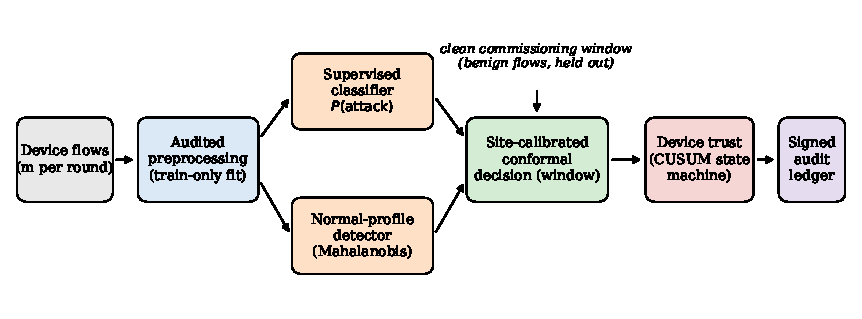
\includegraphics[width=0.9\textwidth]{framework.pdf}
\caption{Framework: audited preprocessing, two scorers, site-calibrated conformal decision, CUSUM device trust and signed audit ledger.}
\label{fig:framework}
\end{figure*}

\subsection{System Model and Notation}
A flow is described by a feature vector $\mathbf{x}\in\mathbb{R}^{d}$ and a label $y\in\{0,\dots,K-1\}$ where class $0$ is Normal. Each device emits $m$ flows per inference round. The site provides a commissioning window $\mathcal{W}$ of $n$ flows known to be benign. The threat model assumes that the window is clean, that benign traffic after commissioning is exchangeable with it, that an attacker can modify the log store but cannot read the signing key, and that the head digest of the ledger is periodically copied to a witness store outside the attacker's reach. Table~\ref{tab:notation} lists the notation.

\begin{table}[t]
\centering
\caption{Notation.}
\label{tab:notation}
\footnotesize
\setlength{\tabcolsep}{3pt}
\resizebox{\columnwidth}{!}{%
\begin{tabular}{@{}ll@{}}
\toprule
Symbol & Meaning \\
\midrule
$\mathbf{x},y,K$ & flow features, label, number of classes (class 0 is Normal) \\
$p_k(\mathbf{x})$ & classifier posterior of class $k$ \\
$s_c(\mathbf{x})=1-p_0(\mathbf{x})$ & classifier attack score \\
$s_a(\mathbf{x})$ & Normal-profile anomaly score \\
$\mathcal{W},n$ & commissioning window and its size \\
$\alpha,\tau_\alpha$ & target benign false-alarm rate and conformal threshold \\
$m,t$ & flows per round, round index \\
$\mathbf{w},w_u$ & class severity weights, severity of an unknown anomaly \\
$x_t$ & round evidence in $[0,1]$ \\
$\mu_0,\kappa,h,c$ & CUSUM baseline, allowance, threshold and cap factor \\
$S_t,T_t$ & CUSUM statistic and trust score \\
$\mu_b,\mu_a$ & mean evidence of a benign and of a compromised device \\
$m_{\mathrm{eff}}$ & effective number of independent flows per round \\
\bottomrule
\end{tabular}}
\end{table}

\subsection{Audited Data Protocol}
Official partitions are kept when they exist (NSL-KDD, UNSW-NB15), and a stratified 80/20 split is used otherwise (Edge-IIoTset). Exact duplicate records are removed, and test records identical to a training record are dropped and counted. A 15\% validation set is carved from the remaining training records before any resampling. Category vocabularies, the scaler, feature selection and resampling are fitted on the training partition only. The label-conditioned difficulty attribute of NSL-KDD is never used as a feature. Standardized features are clipped to $[-5,5]$, because rare-event attributes reach standardized values above 100 in NSL-KDD and destabilized batch-normalized networks. Features are selected by class-aware mutual information: for each class the mutual information between every feature and the one-versus-rest label is normalized by its maximum, and the score of a feature is its maximum over classes, which keeps rare-class indicators that a global ranking discards. Twenty-five features are kept in canonical attribute order. Training sets are balanced to 4,000 flows per class after the split, by random undersampling and SMOTE.

\subsection{Classifier and Normal-Profile Detector}
LightGBM with 300 trees, learning rate 0.05 and 31 leaves is the primary classifier. The Normal-profile detector is fitted on Normal training flows only, using all standardized features. Its score is the squared Mahalanobis distance
\begin{equation}
s_a(\mathbf{x})=(\mathbf{x}-\hat{\boldsymbol{\mu}})^{\top}\hat{\boldsymbol{\Sigma}}^{-1}(\mathbf{x}-\hat{\boldsymbol{\mu}}),
\label{eq:maha}
\end{equation}
where $\hat{\boldsymbol{\mu}}$ is the mean of the Normal flows and $\hat{\boldsymbol{\Sigma}}$ is the Ledoit-Wolf shrinkage covariance \cite{ledoit2004well}. A Gaussian profile was chosen because it has few degrees of freedom and a closed-form score, which keeps the score distribution of shifted benign traffic close to that of the training benign traffic. Equation~\eqref{eq:maha} measures how far a flow lies from the benign profile in units of the benign covariance. Isolation Forest \cite{liu2008isolation} is evaluated as an alternative.

\subsection{Site-Calibrated Conformal Decision}
An argmax decision uses an operating point validated on the training distribution. Under shift the benign false-alarm rate can move far from that point. Calibrating on a clean window of the site controls the rate directly. For a score $s$ and a commissioning window of $n$ benign flows with scores $s_{(1)}\le\dots\le s_{(n)}$, the split-conformal threshold \cite{vovk2005algorithmic,bates2023testing} is
\begin{equation}
\tau_\alpha=s_{(\lceil (n+1)(1-\alpha)\rceil)},\qquad \Pbb\big[s(\mathbf{x})>\tau_\alpha\big]\le\alpha,
\label{eq:conformal}
\end{equation}
for any benign $\mathbf{x}$ exchangeable with the window, because the rank of a new benign score among $n+1$ exchangeable scores is uniform. The threshold exists only if $n\ge\lceil(1-\alpha)/\alpha\rceil$, which is 19 flows for $\alpha=5\%$ and 49 flows for $\alpha=2\%$. The classifier decision then becomes
\begin{equation}
\hat{y}(\mathbf{x})=\begin{cases}0,& s_c(\mathbf{x})\le\tau_\alpha,\\ \arg\max_{k\ne0}p_k(\mathbf{x}),& \text{otherwise.}\end{cases}
\label{eq:decision}
\end{equation}
Equation~\eqref{eq:decision} keeps the learned ranking of attack classes and replaces only the Normal-versus-attack boundary. The guarantee is marginal and holds for the false-alarm rate on benign traffic, not for attack recall, and it requires that benign traffic after commissioning stays exchangeable with the window. For fusion, a flow is declared an attack if the classifier or the detector raises it, with the detector threshold set by Eq.~\eqref{eq:conformal}, and a flow raised only by the detector receives the most probable attack class. For matched-rate comparisons, scores are converted to ranks $F_c,F_a$ relative to the window and combined as $u=\max\{F_c(s_c),F_a(s_a)\}$, and the threshold of $u$ is again set by Eq.~\eqref{eq:conformal}. Algorithm~\ref{alg:site} summarizes the procedure.

\begin{algorithm}[t]
\caption{Site calibration and decision.}
\label{alg:site}
\begin{algorithmic}[1]
\REQUIRE trained classifier, Normal-profile detector, clean window $\mathcal{W}$ of $n$ flows, target $\alpha$
\STATE compute $s_c$ and $s_a$ on $\mathcal{W}$; verify $n\ge\lceil(1-\alpha)/\alpha\rceil$, else report that no threshold exists
\STATE set $\tau^{c}_\alpha$ and $\tau^{a}_\alpha$ by Eq.~\eqref{eq:conformal}
\FOR{each new flow $\mathbf{x}$}
\STATE $\hat{y}\leftarrow$ Eq.~\eqref{eq:decision} with $\tau^{c}_\alpha$
\IF{$\hat{y}=0$ and $s_a(\mathbf{x})>\tau^{a}_\alpha$}
\STATE $\hat{y}\leftarrow\arg\max_{k\ne0}p_k(\mathbf{x})$; mark flow as detector-only
\ENDIF
\ENDFOR
\end{algorithmic}
\end{algorithm}

\subsection{Class-Aware Device Trust}
The round evidence of a device aggregates severity-weighted harm over its $m$ flows,
\begin{equation}
x_t=\frac{1}{m}\sum_{j=1}^{m}\max\big\{\mathbf{w}^{\top}\mathbf{p}(\mathbf{x}_{tj}),\,w_u z_{tj}\big\},
\label{eq:evidence}
\end{equation}
where $\mathbf{w}=(0,0.6,0.4,0.8,1.0)$ assigns increasing severity to DoS, Probe, R2L and U2R, $z_{tj}\in\{0,1\}$ flags a detector-only anomaly and $w_u=0.5$. Unlike a confidence-only rule, Eq.~\eqref{eq:evidence} gives no credit to a confident attack prediction. A one-sided CUSUM statistic with a cap accumulates the excess over a baseline,
\begin{align}
S_t&=\min\{ch,\ \max(0,\ S_{t-1}+x_t-\mu_0-\kappa)\},\label{eq:cusum}\\
T_t&=\max(0,\ 1-S_t/h).\nonumber
\end{align}
The baseline $\mu_0$ is the mean evidence of the device over a commissioning period of $W$ rounds, or the fleet median of these means. A device is Healthy when $S_t\le0.25h$, Quarantined when $S_t\ge h$ and released when $S_t\le0.5h$, and Degraded otherwise. The cap bounds the recovery time after an attack ends.

For a benign device with mean evidence $\mu_b$, let $\delta=\kappa+\mu_0-\mu_b>0$. Evidence is a mean of $m_{\mathrm{eff}}$ independent bounded flow terms, so Hoeffding's lemma \cite{hoeffding1963probability} gives $\Ebb\,e^{\theta(x_t-\mu_b)}\le e^{\theta^{2}/(8m_{\mathrm{eff}})}$. With $\theta^{*}=8m_{\mathrm{eff}}\delta$ the process $e^{\theta^{*}S_t}$ is dominated by a supermartingale, which yields
\begin{equation}
\Pbb\big[\exists t:\ S_t\ge h\big]\le e^{-8m_{\mathrm{eff}}\delta h}.
\label{eq:fq}
\end{equation}
The cap only lowers $S_t$ and leaves the bound valid. For a compromised device with mean evidence $\mu_a>\mu_0+\kappa$, let $d=\mu_a-\mu_0-\kappa$. Wald's identity with an overshoot of at most one gives
\begin{equation}
\Ebb[\tau_Q]\le (h+1)/d,
\label{eq:delay}
\end{equation}
where $\tau_Q$ is the number of rounds to quarantine, and an attack whose flows have mean harm $\mu_{\mathrm{att}}$ is detectable when it occupies a fraction $f$ of flows with $f>f^{*}=(\mu_0+\kappa-\mu_b)/(\mu_{\mathrm{att}}-\mu_b)$. Equation~\eqref{eq:fq} shows how $h$ trades alarms against delay, and Eq.~\eqref{eq:delay} shows that detection fails when the evidence of the attack does not exceed the baseline plus $\kappa$. The threshold is designed as $h=\ln(1/\alpha_q)/(8m\kappa)$, which certifies a false-quarantine probability of at most $\alpha_q$ when $\mu_0\approx\mu_b$. Algorithm~\ref{alg:trust} gives the update.

\begin{algorithm}[t]
\caption{Device trust update (one device).}
\label{alg:trust}
\begin{algorithmic}[1]
\REQUIRE $m$ flows of round $t$, parameters $\kappa,h,c$, baseline $\mu_0$
\STATE compute $x_t$ by Eq.~\eqref{eq:evidence}
\STATE $S_t\leftarrow\min\{ch,\max(0,S_{t-1}+x_t-\mu_0-\kappa)\}$; $T_t\leftarrow\max(0,1-S_t/h)$
\IF{state is Quarantined}
\STATE release to Degraded or Healthy only if $S_t\le0.5h$
\ELSE
\STATE state $\leftarrow$ Quarantined if $S_t\ge h$, Healthy if $S_t\le0.25h$, else Degraded
\ENDIF
\STATE append $(\text{device},t,T_t,\text{state})$ to the ledger
\end{algorithmic}
\end{algorithm}

\subsection{Signed and Anchored Audit Ledger}
The ledger is an append-only log with a single writer. Block $i$ stores a timestamp $t_i$, a payload $r_i$ and the digest $H_i=\mathrm{SHA256}(i\,\|\,t_i\,\|\,r_i\,\|\,H_{i-1})$, and the writer signs $H_i$ with Ed25519 \cite{bernstein2012high}. Every 50 blocks the head digest is copied to a witness store. Verification recomputes all digests, checks all signatures and compares the witness digests with the chain. A plain hash chain detects only in-place edits, because an attacker who can rewrite the store can recompute all later digests. Signatures remove this option for attackers without the key, and witness digests detect rewrites by a key holder, with truncation detected only if it removes an anchored block. The ledger has no consensus, no replicas and no smart contracts, and it is therefore described as an audit log and not as a blockchain.

\subsection{Differentially Private Training}
The privacy baseline trains a LayerNorm CNN-BiLSTM with DP-SGD: Poisson sampling with rate $q=B/N$, per-example gradient clipping to norm $C=1$, Gaussian noise of standard deviation $\sigma C$, and a R\'enyi accountant for the sampled Gaussian mechanism \cite{mironov2019sampled} converted to $(\varepsilon,\delta)$ with $\delta=1/N$. The noise multiplier is calibrated by bisection for a target $\varepsilon$, and the accountant was verified against an independent implementation to four decimals. The neighboring relation adds or removes one original training record, and training uses the original records without oversampling so that one record cannot influence many rows. Preprocessing, class weights and hyper-parameter choices are outside the guarantee. Laplace noise added to inputs without a sensitivity bound is not claimed as differential privacy.

\subsection{Baselines}
Random forest (300 trees), MLP, CNN, LSTM and CNN-BiLSTM treat the 25 selected features as a length-25 sequence in canonical attribute order. The CNN-BiLSTM has two convolutional layers (256 and 128 filters, kernel 3) with LayerNorm and dropout, a bidirectional LSTM with 128 units, and dense layers of 256 and 128 units (462,725 parameters). The dual-attention variant adds channel and temporal attention (471,205 parameters) and approximates, without reproducing, the architecture of ZT-DT \cite{mishra2026zero}. Baselines differ from the proposed pipeline only in the classifier, and all share the same data, features, seeds and hardware.

\subsection{Computational Complexity}
Preprocessing costs $O(d)$ per flow. Mahalanobis scoring costs $O(d^{2})$ per flow with $d=122$, and conformal calibration costs $O(n\log n)$ once per site. LightGBM inference costs $O(T\,\ell)$ for $T=300$ trees of depth $\ell$, and the CNN-BiLSTM costs $O(L(c\,d\,k_s+u^{2}))$ with sequence length $L=25$, $c$ filters, kernel $k_s$ and $u$ recurrent units. The trust update costs $O(m)$ per device round, and a ledger append costs $O(1)$ for the digest and one signature. Verification is $O(N)$ in the chain length. Isolation Forest scoring would cost $O(T_f\log\psi)$ per flow for $T_f$ trees and subsample size $\psi$, which is lower than the quadratic Mahalanobis cost but gave a lower ranking quality on all datasets with a per-flow output.

\begin{table}[t]
\centering
\caption{Parameters and their justification.}
\label{tab:params}
\setlength{\tabcolsep}{3pt}
\footnotesize
\begin{tabular}{@{}p{2.3cm}p{1.6cm}p{3.7cm}@{}}
\toprule
Parameter & Value & Justification \\
\midrule
Target $\alpha$ & 2, 5, 10\% & all reported; chosen from the alarm budget \\
Commissioning window & 10\% of benign test flows & held out; 20 random windows \\
Clip of standardized features & $[-5,5]$ & rare-event attributes reach $|z|>100$ \\
Selected features & 25 & matches the sequence baselines \\
Flows per round $m$ & 20 & small enough for per-round latency \\
Allowance $\kappa$ & 0.05 & margin above baseline estimation error \\
Threshold $h$ & 0.576 & $\ln(100)/(8\cdot20\cdot0.05)$, $\alpha_q=1\%$ \\
Cap factor $c$ & 2 & bounds recovery time \\
Commissioning rounds $W$ & 10 & clean at the start of every scenario \\
Severity $\mathbf{w}$, $w_u$ & see text & policy table, configurable \\
Anchor interval & 50 blocks & cost of one copy per 50 appends \\
DP clip, $\delta$ & 1, $1/N$ & standard practice \\
\bottomrule
\end{tabular}
\end{table}

\section{Experimental Protocol}\label{sec:setup}
NSL-KDD \cite{tavallaee2009detailed} and UNSW-NB15 \cite{moustafa2015unsw} use their official training and testing partitions, and Edge-IIoTset \cite{ferrag2022edge} uses the file prepared for machine learning with a stratified split. For Edge-IIoTset, identifiers and payload fields are excluded, and a second run additionally removes capture-related fields (TCP sequence and acknowledgment numbers and checksums, ICMP checksum and sequence), to measure how many records differ only in those fields. Every stochastic result is the mean and sample standard deviation over three training seeds (0, 1 and 2). Seeds change the validation split, the resampling and the initialization, whereas the official test partitions are fixed, so the standard deviations reflect training randomness only. Per-class recall uses the proportion of correctly classified test flows. For the site-calibrated results, the commissioning window is a random 10\% of the benign test flows, excluded from the evaluation, and values are means over 20 windows (10 for the leave-one-class-out test). The leave-one-class-out test trains LightGBM without one attack class and compares the classifier score, the detector score and their rank maximum, each at the same benign false-alarm rate, together with the threshold-free area under the ROC curve (AUROC). Trust experiments replay real test-set evidence into 200 simulated devices per scenario, with 60 rounds of $m=20$ flows, and the flows of a round are sampled independently. Latency is measured with one thread on an 8-core Windows 11 machine. Training and test partitions for the trust replay come from the same classifier outputs as the detection results.

\section{Results}\label{sec:results}
\subsection{Benchmark Audit}
Duplicated records are common in all three benchmarks and differ in kind. In NSL-KDD only 16 training records are duplicates, but 664 of the 22,544 test records (2.9\%) are identical to a training record. In UNSW-NB15, 74,301 of 175,341 training records (42.4\%) are exact duplicates and 8,541 of 82,332 test records (10.4\%) equal a training record. In Edge-IIoTset 5,726 of 157,800 records (3.6\%) are exact duplicates, but removing capture-related fields turns 141,514 records (89.7\%) into duplicates and leaves 16,286 unique records with only 397 Normal flows, so many Edge-IIoTset records differ only in capture artifacts. Table~\ref{tab:audit} lists the counts. A random split of such a corpus places near-copies on both sides, and scores obtained that way describe memorization as well as detection.

\begin{table*}[t]
\centering
\caption{Duplicate audit of the three benchmarks.}
\label{tab:audit}
\small
\resizebox{\textwidth}{!}{\begin{tabular}{lcccc}
\toprule
Benchmark & Records (train + test) & Exact duplicates & Test rows equal to a training row & Train+val / test after audit \\
\midrule
NSL-KDD (official split) & 125,973 + 22,544 & 16 (0.01\%) & 664 (2.9\%) & 125,957 / 21,833 \\
UNSW-NB15 (official split) & 175,341 + 82,332 & 74,301 (42.4\%) & 8,541 (10.4\%) & 101,040 / 52,644 \\
Edge-IIoTset (random split) & 157,800 & 5,726 (3.6\%) & -- & 96,000 / 24,000 \\
Edge-IIoTset, capture fields removed & 157,800 & 141,514 (89.7\%) & -- & 13,021 / 3,256 \\
\bottomrule
\end{tabular}
}
\end{table*}

\subsection{Detection on the Audited NSL-KDD Protocol}
LightGBM with class-aware features reaches a macro-F1 of $0.634\pm0.024$ and an accuracy of $0.776\pm0.019$, whereas the CNN-BiLSTM reaches $0.554\pm0.018$ and $0.745\pm0.010$ (Table~\ref{tab:main}). Random forest, MLP, CNN and LSTM obtain macro-F1 values between 0.522 and 0.566, so the deep sequence models do not improve over gradient boosting or over a plain MLP, and equal-weight averaging of LightGBM and CNN-BiLSTM posteriors gives $0.636\pm0.007$, which is within the seed variation of LightGBM alone. Dual attention lowers macro-F1 from 0.554 to 0.542, and the feature order has no measurable effect (canonical 0.554, random 0.557, descending mutual information 0.561), which does not support the premise that recurrent layers exploit sequential structure in flow features. Class-aware feature selection improves LightGBM from $0.562\pm0.009$ to $0.634\pm0.024$ macro-F1 and R2L recall from 0.076 to 0.191, whereas global mutual information discards the rare-class indicators.

\begin{table*}[t]
\centering
\caption{NSL-KDD, official overlap-free test set, mean $\pm$ standard deviation over seeds.}
\label{tab:main}
\scriptsize
\setlength{\tabcolsep}{3pt}
\resizebox{\textwidth}{!}{\begin{tabular}{lccccccc}
\toprule
Model & Acc. & Macro-F1 & MCC & Normal FPR & R2L rec. & U2R rec. & Seeds \\
\midrule
CNN-BiLSTM + class-aware MI (proposed) & 0.745$\pm$0.010 & 0.554$\pm$0.018 & 0.620$\pm$0.018 & 0.081$\pm$0.029 & 0.183$\pm$0.041 & 0.527$\pm$0.031 & 3 \\
CNN-BiLSTM + dual attention & 0.739$\pm$0.021 & 0.542$\pm$0.027 & 0.610$\pm$0.035 & 0.075$\pm$0.026 & 0.131$\pm$0.061 & 0.537$\pm$0.117 & 3 \\
CNN-BiLSTM + global MI (original selection) & 0.728$\pm$0.006 & 0.514$\pm$0.002 & 0.597$\pm$0.009 & 0.104$\pm$0.001 & 0.165$\pm$0.007 & 0.418$\pm$0.039 & 3 \\
LightGBM (class-aware MI, 25 feat.) & 0.776$\pm$0.019 & 0.634$\pm$0.024 & 0.675$\pm$0.026 & 0.029$\pm$0.002 & 0.191$\pm$0.004 & 0.408$\pm$0.075 & 3 \\
LightGBM (global MI, 25 feat.) & 0.775$\pm$0.011 & 0.562$\pm$0.009 & 0.672$\pm$0.017 & 0.030$\pm$0.001 & 0.076$\pm$0.012 & 0.264$\pm$0.023 & 3 \\
LightGBM (all features) & 0.775 & 0.624 & 0.674 & 0.028 & 0.222 & 0.269 & 1 \\
Random forest (class-aware MI) & 0.752$\pm$0.002 & 0.566$\pm$0.018 & 0.639$\pm$0.003 & 0.029$\pm$0.001 & 0.077$\pm$0.007 & 0.294$\pm$0.075 & 3 \\
MLP & 0.752$\pm$0.014 & 0.560$\pm$0.028 & 0.633$\pm$0.023 & 0.077$\pm$0.028 & 0.148$\pm$0.052 & 0.537$\pm$0.026 & 3 \\
CNN only & 0.735$\pm$0.016 & 0.549$\pm$0.041 & 0.604$\pm$0.025 & 0.102$\pm$0.003 & 0.174$\pm$0.099 & 0.642$\pm$0.015 & 3 \\
LSTM only & 0.731$\pm$0.018 & 0.522$\pm$0.055 & 0.601$\pm$0.022 & 0.091$\pm$0.024 & 0.099$\pm$0.074 & 0.582$\pm$0.113 & 3 \\
\bottomrule
\end{tabular}
}
\end{table*}

The gap between protocols is large. On a deduplicated random split LightGBM reaches an accuracy of $0.988\pm0.001$ and a macro-F1 of $0.878\pm0.013$, against $0.776$ and $0.634$ on the official split, so random splits overstate performance by 0.24 macro-F1 points. The remaining errors concentrate in few sub-types. The R2L sub-type guess\_passwd contributes 1,231 test flows and none of them is recognized, although it is present in training. The 53 training examples are all telnet sessions with failed logins, whereas most test examples target pop\_3 or ftp with successful logins, so the test examples differ from every training example. No weighting scheme can recover this, and weighting by sub-type was tried and did not help. The targeted poisoning of 50\% of the R2L and U2R labels lowers R2L recall from 0.183 to 0.054 and U2R recall from 0.527 to 0.204, whereas random noise on 30\% of the labels leaves macro-F1 unchanged (0.555).

\subsection{Site-Calibrated Decisions}
Table~\ref{tab:site} compares the argmax decision with the site-calibrated rule of Eq.~\eqref{eq:decision}. On UNSW-NB15 the argmax decision labels 38.6\% of benign flows as attacks, and calibration at $\alpha=5\%$ gives a measured rate of $0.050\pm0.000$, raises accuracy from $0.677$ to $0.818$ and macro-F1 from 0.526 to 0.549, at the cost of attack detection falling from 0.989 to 0.755. On NSL-KDD the same target raises accuracy from $0.767$ to $0.813$ and macro-F1 from $0.632$ to $0.660$, with a measured rate of 0.050. On Edge-IIoTset, where the argmax decision already has no benign false alarms, calibration costs 0.008 macro-F1 at $\alpha=5\%$. The measured benign rates equal the targets within 0.004 for all three datasets and all three levels, which agrees with Eq.~\eqref{eq:conformal}. A strict target is not always better: at $\alpha=2\%$ NSL-KDD macro-F1 falls to 0.466, because the classifier assigns inflated attack probabilities to shifted benign traffic and the rule then rejects many attacks. The benefit therefore depends on how far the argmax operating point lies from the intended one.

\begin{table}[t]
\centering
\caption{LightGBM decision: argmax versus site-calibrated threshold.}
\label{tab:site}
\scriptsize
\setlength{\tabcolsep}{3pt}
\resizebox{\columnwidth}{!}{\begin{tabular}{llcccc}
\toprule
Dataset & Decision rule & Acc. & Macro-F1 & Benign FPR & Attack det. \\
\midrule
NSL-KDD & argmax & 0.767$\pm$0.020 & 0.632$\pm$0.025 & 0.029$\pm$0.002 & 0.658$\pm$0.047 \\
NSL-KDD & site, $\alpha=0.02$ & 0.685$\pm$0.016 & 0.466$\pm$0.034 & 0.019$\pm$0.002 & 0.485$\pm$0.029 \\
NSL-KDD & site, $\alpha=0.05$ & 0.813$\pm$0.007 & 0.660$\pm$0.021 & 0.050$\pm$0.002 & 0.787$\pm$0.029 \\
NSL-KDD & site, $\alpha=0.10$ & 0.819$\pm$0.003 & 0.651$\pm$0.022 & 0.100$\pm$0.001 & 0.889$\pm$0.021 \\
UNSW-NB15 & argmax & 0.677$\pm$0.002 & 0.526$\pm$0.006 & 0.386$\pm$0.005 & 0.989$\pm$0.004 \\
UNSW-NB15 & site, $\alpha=0.02$ & 0.816$\pm$0.002 & 0.542$\pm$0.004 & 0.020$\pm$0.001 & 0.676$\pm$0.011 \\
UNSW-NB15 & site, $\alpha=0.05$ & 0.818$\pm$0.003 & 0.549$\pm$0.002 & 0.050$\pm$0.000 & 0.755$\pm$0.013 \\
UNSW-NB15 & site, $\alpha=0.10$ & 0.807$\pm$0.003 & 0.550$\pm$0.004 & 0.100$\pm$0.000 & 0.836$\pm$0.012 \\
Edge-IIoTset & argmax & 0.941$\pm$0.001 & 0.913$\pm$0.001 & 0.000$\pm$0.000 & 1.000$\pm$0.000 \\
Edge-IIoTset & site, $\alpha=0.02$ & 0.939$\pm$0.000 & 0.911$\pm$0.001 & 0.018$\pm$0.000 & 1.000$\pm$0.000 \\
Edge-IIoTset & site, $\alpha=0.05$ & 0.934$\pm$0.000 & 0.905$\pm$0.000 & 0.052$\pm$0.002 & 1.000$\pm$0.000 \\
Edge-IIoTset & site, $\alpha=0.10$ & 0.927$\pm$0.000 & 0.897$\pm$0.000 & 0.102$\pm$0.004 & 1.000$\pm$0.000 \\
\bottomrule
\end{tabular}
}
\end{table}

\subsection{Novelty Fusion and Its Transfer}
The Normal-profile detector helps on NSL-KDD, where the test partition contains 17 attack sub-types that are absent from training (3,695 of 12,251 attacks). Table~\ref{tab:novelty} shows that fusing the Mahalanobis detector with a validation threshold raises macro-F1 from 0.634 to $0.704\pm0.022$ and the detection of unseen-type attacks from 0.30 to 0.59, at 3.5\% benign false alarms. Calibrating the detector threshold on the commissioning window gives $0.707\pm0.004$ and 0.63 with a benign rate of 3.8\%, and it raises R2L recall from 0.19 to $0.434\pm0.061$ because flagged flows receive the most probable attack class. Mahalanobis ranks the attacks better than Isolation Forest, with an AUROC of 0.966 against 0.942, and the same order holds on UNSW-NB15 (0.726 against 0.679) and Edge-IIoTset (1.000 against 0.829) in the leave-one-class-out test. The choice of Mahalanobis and of site calibration was made after inspecting NSL-KDD results, which is why the next test uses other data.

\begin{table}[t]
\centering
\caption{NSL-KDD: LightGBM with Normal-profile fusion.}
\label{tab:novelty}
\scriptsize
\setlength{\tabcolsep}{2.5pt}
\resizebox{\columnwidth}{!}{\begin{tabular}{lcccccc}
\toprule
Configuration & Macro-F1 & Benign FPR & Det. seen & Det. unseen & R2L rec. & U2R rec. \\
\midrule
LightGBM alone & 0.634$\pm$0.024 & 0.029$\pm$0.002 & 0.814$\pm$0.015 & 0.297$\pm$0.135 & 0.191$\pm$0.004 & 0.408$\pm$0.075 \\
+ IsolationForest (validation threshold) & 0.667$\pm$0.029 & 0.032$\pm$0.002 & 0.818$\pm$0.012 & 0.583$\pm$0.062 & 0.195$\pm$0.005 & 0.458$\pm$0.099 \\
+ Mahalanobis (validation threshold) & 0.704$\pm$0.022 & 0.035$\pm$0.002 & 0.894$\pm$0.031 & 0.592$\pm$0.020 & 0.351$\pm$0.033 & 0.562$\pm$0.135 \\
LightGBM alone, commissioning flows excluded & 0.632$\pm$0.025 & 0.029$\pm$0.002 & 0.814$\pm$0.015 & 0.297$\pm$0.135 & 0.191$\pm$0.004 & 0.408$\pm$0.075 \\
+ Mahalanobis (site, conformal) & 0.707$\pm$0.004 & 0.038$\pm$0.001 & 0.941$\pm$0.005 & 0.630$\pm$0.008 & 0.434$\pm$0.061 & 0.562$\pm$0.135 \\
\bottomrule
\end{tabular}
}
\end{table}

Table~\ref{tab:loo} reports the leave-one-attack-class-out test at matched false-alarm rates. On UNSW-NB15 the classifier trained without a class still ranks it well (AUROC $0.921\pm0.057$), the detector ranks it worse (0.726), and the fused score does not improve on the classifier (0.903 and a detection rate of 0.505 against 0.527 at about 5\% benign false alarms). On Edge-IIoTset the classifier alone separates every held-out class (AUROC 1.000), so the test cannot reveal a benefit. The novelty gain is therefore specific to NSL-KDD, where unseen sub-types are variants of seen families that the classifier misses, and it is not established for datasets whose attack classes are already well separated from Normal.

\begin{table}[t]
\centering
\caption{Leave-one-attack-class-out at matched benign false-alarm rate (5\%).}
\label{tab:loo}
\scriptsize
\setlength{\tabcolsep}{2.5pt}
\resizebox{\columnwidth}{!}{\begin{tabular}{lccccccc}
\toprule
Dataset & Classes & AUROC clf & AUROC det & AUROC fused & Det. clf & Det. det & Det. fused \\
\midrule
UNSW-NB15 & 5 & 0.921$\pm$0.057 & 0.726$\pm$0.153 & 0.903$\pm$0.070 & 0.527$\pm$0.301 & 0.185$\pm$0.177 & 0.505$\pm$0.263 \\
Edge-IIoTset & 5 & 1.000$\pm$0.000 & 1.000$\pm$0.000 & 0.998$\pm$0.001 & 1.000$\pm$0.000 & 1.000$\pm$0.000 & 1.000$\pm$0.000 \\
\bottomrule
\end{tabular}
}
\end{table}

\subsection{Device Trust Under Multi-Round Scenarios}
The confidence-only update of the first version detects none of the compromised devices, because a confident attack prediction raises the score, whereas the class-aware CUSUM rule detects all of them with a median delay of two rounds and no false quarantine on a homogeneous fleet (Table~\ref{tab:trust}). The beta-reputation rule detects 72\% of the devices with a median delay of eight rounds and none of the attacks of unseen types, which only the evidence with novelty flags covers. On a heterogeneous fleet, in which devices differ in service, a shared fleet baseline with classifier evidence quarantines 18.5\% of the benign devices, and per-device baselines remove all false quarantines. Figure~\ref{fig:trust} shows that a repaired device is released after the attack ends and that intermittent bursts keep a device quarantined. When 10\% to 45\% of the fleet is already compromised during commissioning, the fleet-median baseline still detects all of them, whereas per-device baselines detect at most about 2\%, because the attack is absorbed into the baseline. A scan of 29 settings of $\kappa$, $\alpha_q$, $m$ and the commissioning length gives no false quarantine, detection of every compromised device and 70\% to 100\% detection of attacks with 30\% intensity.

\begin{table*}[t]
\centering
\caption{Trust update rules on replayed evidence.}
\label{tab:trust}
\scriptsize
\resizebox{\textwidth}{!}{\begin{tabular}{llccccc}
\toprule
Fleet & Rule & False quar. (\%) & Detect (\%) & Delay & Unseen type (\%) & Stealth 30\% (\%) \\
\midrule
Homogeneous & Confidence-only & 0.0 & 0 & -- & 0 & 0 \\
Homogeneous & Beta reputation & 0.0 & 72 & 8 & 0 & 0 \\
Homogeneous & CUSUM, fleet baseline & 0.0 & 100 & 2 & 100 & 97 \\
Homogeneous & CUSUM, device baseline, +novelty & 0.0 & 100 & 2 & 100 & 96 \\
Heterogeneous & Confidence-only & 0.0 & 0 & -- & 0 & 0 \\
Heterogeneous & Beta reputation & 0.0 & 76 & 8 & 0 & 0 \\
Heterogeneous & CUSUM, fleet baseline & 18.5 & 100 & 2 & 100 & 82 \\
Heterogeneous & CUSUM, device baseline, +novelty & 0.0 & 100 & 2 & 100 & 88 \\
\bottomrule
\end{tabular}
}
\end{table*}

\begin{figure*}[t]
\centering
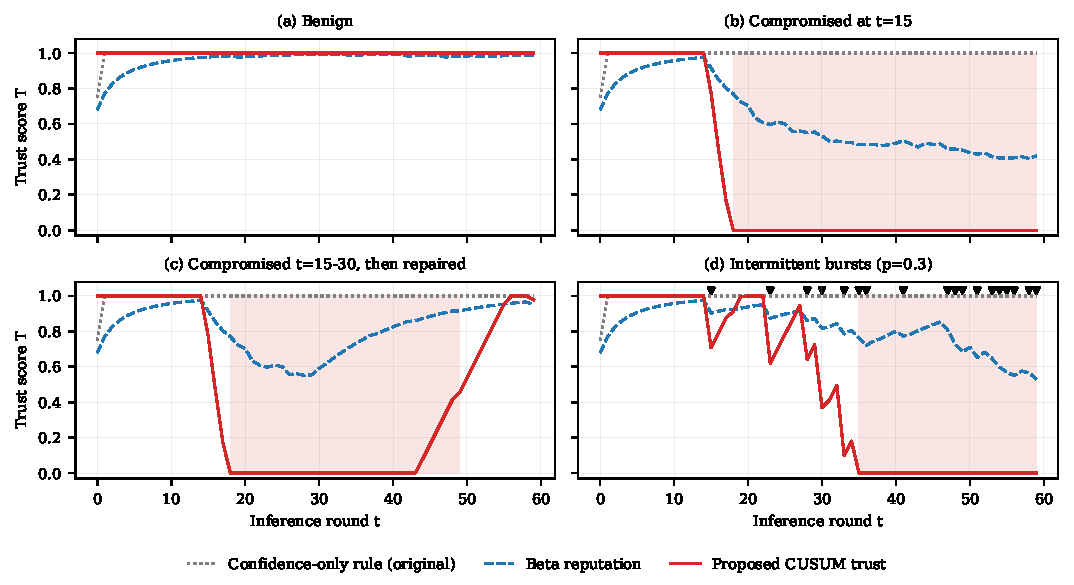
\includegraphics[width=0.85\textwidth]{trust_trajectories.pdf}
\caption{Trust trajectories for benign, compromised, repaired and intermittent devices.}
\label{fig:trust}
\end{figure*}

The bounds of Eq.~\eqref{eq:fq} and Eq.~\eqref{eq:delay} held empirically (Fig.~\ref{fig:theory}). The observed false-quarantine rate did not exceed the certified level in any of 12 settings, including settings in which flows within a round were correlated and $m_{\mathrm{eff}}$ was reduced. The measured mean delays were 1.98, 2.00, 3.40 and 1.29 rounds for DoS, Probe, R2L and U2R, against bounds of 3.46, 3.71, 7.84 and 2.49. Detection of a mixed round switches on near the predicted fraction $f^{*}$ (0.099 for DoS and 0.199 for R2L). These experiments replay classifier outputs and sample flows independently, so they validate the update rule and not an end-to-end deployment.

\begin{figure*}[t]
\centering
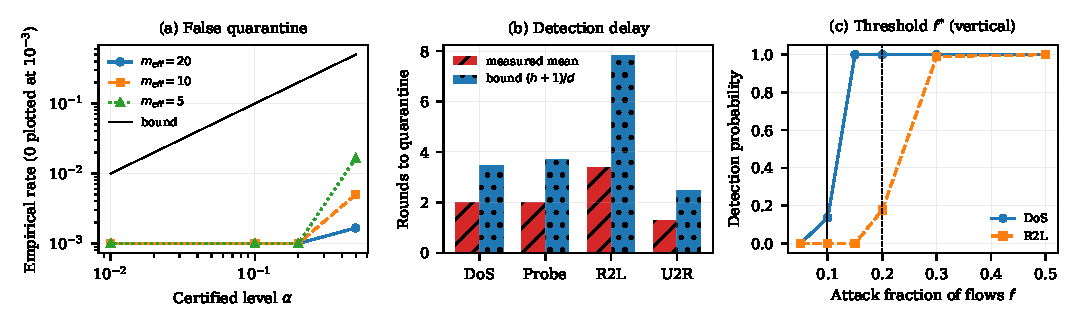
\includegraphics[width=0.95\textwidth]{trust_theory.pdf}
\caption{Validation of the false-quarantine bound, the delay bound and the minimum detectable fraction.}
\label{fig:theory}
\end{figure*}

\subsection{Audit Ledger and Privacy}
The plain hash chain detected only the in-place edit without re-hashing, and signatures added detection of edits, deletions and rewrites by attackers without the key (Table~\ref{tab:ledger}). Edits by a key holder were detected at 93.5\% with witness anchors, and truncation at 50\%, which is the fraction of truncations that removed an anchored block. Mean detection over the six attacks rose from 16.7\% to 66.7\% and to 90.6\%. A signed append cost 51.7 $\mu$s against 10.2 $\mu$s for a digest alone, and verifying 10,000 blocks took 1.11 s.

\begin{table}[t]
\centering
\caption{Tamper detection rate (\%) of the ledger variants.}
\label{tab:ledger}
\scriptsize
\setlength{\tabcolsep}{2.5pt}
\resizebox{\columnwidth}{!}{\begin{tabular}{lccc}
\toprule
Attack & hash chain only & + signatures & + signatures + anchors \\
\midrule
edit\_no\_rehash & 100.0 & 100.0 & 100.0 \\
edit\_rehash\_no\_key & 0.0 & 100.0 & 100.0 \\
edit\_rehash\_with\_key & 0.0 & 0.0 & 93.5 \\
delete\_relink\_no\_key & 0.0 & 100.0 & 100.0 \\
truncate\_with\_key & 0.0 & 0.0 & 50.0 \\
rewrite\_own\_key & 0.0 & 100.0 & 100.0 \\
untampered chain accepted & yes & yes & yes \\
\bottomrule
\end{tabular}
}
\end{table}

DP-SGD reduces macro-F1 from 0.624 for the same architecture without noise to between 0.448 and 0.475 for $\varepsilon$ from 50 to 1 (Table~\ref{tab:dp}), and U2R recall falls from 0.34 to zero at every $\varepsilon$, because 44 training examples cannot be learned once each example is clipped and noise is added. The membership-inference AUC of a loss-threshold attack is between 0.49 and 0.50 for all models including the non-private one, so this attack provides no empirical evidence of leakage either way, and the claim rests on the accountant.

\begin{table}[t]
\centering
\caption{DP-SGD privacy-utility trade-off, single seed.}
\label{tab:dp}
\scriptsize
\setlength{\tabcolsep}{2.5pt}
\resizebox{\columnwidth}{!}{\begin{tabular}{lcccccc}
\toprule
$\varepsilon$ & $\sigma$ & Acc. & Macro-F1 & MCC & U2R rec. & MIA AUC \\
\midrule
non-private & -- & 0.775 & 0.624 & 0.670 & 0.343 & 0.492 \\
50.00 & 0.34 & 0.744 & 0.475 & 0.620 & 0.000 & 0.497 \\
25.00 & 0.36 & 0.745 & 0.471 & 0.621 & 0.000 & 0.495 \\
8.00 & 0.49 & 0.734 & 0.453 & 0.604 & 0.000 & 0.494 \\
4.00 & 0.59 & 0.724 & 0.449 & 0.590 & 0.000 & 0.496 \\
1.00 & 0.96 & 0.718 & 0.448 & 0.587 & 0.000 & 0.496 \\
\bottomrule
\end{tabular}
}
\end{table}

\subsection{Explainability and Cost}
SHAP attributions of the CNN-BiLSTM were computed on 867 class-stratified flows with named features. Masking the five most attributed features lowers the predicted-class probability by 0.517, against 0.172 for random features, so the attributions are faithful to the network (Fig.~\ref{fig:shap}). The attributions of the CNN-BiLSTM and of a LightGBM surrogate agree weakly (Spearman 0.234, $p=0.261$), which indicates that the two models rely on different features. Interaction values were computed with TreeSHAP on the surrogate, since the SHAP values of the network are not interaction values.

\begin{figure}[t]
\centering
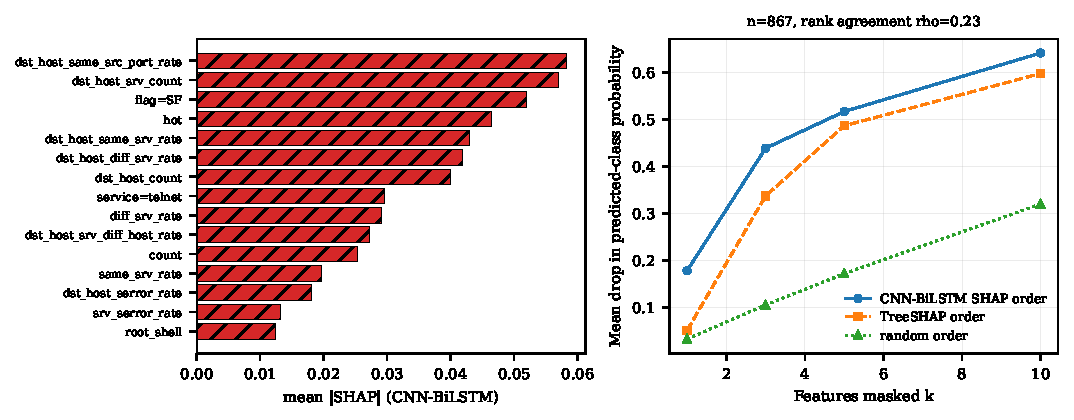
\includegraphics[width=\columnwidth]{shap_faithfulness.pdf}
\caption{SHAP importance and deletion test.}
\label{fig:shap}
\end{figure}

A 20-flow round costs 11.2 ms for CNN-BiLSTM inference, with a 99th percentile of 18.2 ms, and 15.0 ms for preprocessing, inference, trust update and signed ledger append together (Table~\ref{tab:latency}). Against an assumed budget of 100 ms per round, which is a configurable assumption and not a standard, this leaves a factor of 6.7. The attention variant is not slower (13.7 ms per round), so removing attention does not explain a latency reduction. The model occupies 5.6 MB, and a SHAP explanation costs 4.6 s per flow and is therefore an offline function.

\begin{table}[t]
\centering
\caption{Per-round cost on one CPU thread.}
\label{tab:latency}
\scriptsize
\setlength{\tabcolsep}{2pt}
\resizebox{\columnwidth}{!}{\begin{tabular}{lcccccccc}
\toprule
Model & Params & MB & 1 flow (ms) & 20 flows (ms) & p99 (ms) & flows/s & Round total (ms) & Budget margin \\
\midrule
plain & 462,725 & 5.6 & 4.20 & 11.19 & 18.18 & 1631 & 14.99 & 7x \\
attention & 471,205 & 5.7 & 3.57 & 9.88 & 11.33 & 1785 & 13.68 & 7x \\
\bottomrule
\end{tabular}
}
\end{table}

\section{Discussion}\label{sec:discussion}
The results together show that the decision operating point matters more than the architecture. A deep sequence model did not beat gradient boosting on any audited benchmark, the feature order was irrelevant, and the largest gains came from changing how the decision is calibrated and from correcting the evaluation. The audit shows that accuracies measured on random splits of duplicated benchmarks can describe memorization, and the Edge-IIoTset result shows that a small set of capture fields can hide a duplication rate of about 90\% from an exact-duplicate filter.

Three tensions remain. First, novelty fusion helped on NSL-KDD and not on UNSW-NB15, and the test on Edge-IIoTset was uninformative, so a Normal-profile detector should be treated as an option whose value is established per site, with the leave-one-class-out test as the procedure for establishing it. Second, differential privacy and rare classes conflict: at the evaluated budgets the rare class disappears, so privacy protection and detection of rare attacks cannot both be claimed without a design that treats rare classes separately. Third, the trust guarantees assume independent flows and a clean commissioning window, and the replay experiments cannot show how real traffic with temporal dependence behaves, although the correlated-flow stress test did not break the bound.

A practitioner should do four things. Collect a clean commissioning window of at least 19 benign flows per device class, and more if a 2\% target is wanted. Choose $\alpha$ from the alarm budget and not from the best score, since the table shows that the best $\alpha$ depends on the dataset. Use per-device baselines unless the fleet is homogeneous, and use fleet medians when some devices may already be compromised during commissioning. Keep the signing key and the witness digests outside the reach of the log store. The limits of the evidence are a replay simulation for trust, one training configuration for the privacy results, no evaluation on edge hardware, and a leave-one-class-out test that cannot separate the novelty benefit on datasets whose classes are already separable.

\section{Conclusion}\label{sec:conclusion}
This study set out to make IIoT intrusion detection decisions that remain valid at the deployment site, and it audited three public benchmarks to establish a trustworthy basis. The audit found 42.4\% exact duplicates in the UNSW-NB15 training set and 89.7\% duplicates in Edge-IIoTset after capture fields were removed. A zero-trust framework was built on the audited protocol, with a split-conformal site-calibrated decision, a Mahalanobis Normal-profile detector, a class-aware CUSUM trust update and a signed, anchored ledger. Site calibration raised UNSW-NB15 accuracy from 67.7\% to 81.8\% while lowering benign false alarms from 38.6\% to 5.0\%, calibrated fusion raised NSL-KDD macro-F1 from 0.632 to 0.707, and replayed compromised devices were quarantined in a median of two rounds with no false quarantine. The framework met its objective for the decision operating point and for the trust layer, whereas the novelty benefit did not transfer to UNSW-NB15.

The framework applies to sites that can supply a short clean commissioning period, such as plants with a scheduled baseline phase, and its guarantees concern the benign false-alarm rate and the false quarantine of benign devices. A limitation is that the trust results come from replayed evidence and the privacy results from one training configuration. Future work will evaluate the trust layer on time-ordered device traces, repeat the novelty test on datasets with unseen attack variants of seen families, and measure cost and energy on edge hardware. Auditing the data before tuning the model, and calibrating the decision on the site, are low-cost steps that change the reported performance more than the choice of architecture.

\section*{Code Availability}
The code, the result files and the scripts that regenerate every table and figure are available at \url{https://github.com/Al3nzy/Zero_Trust_IIoT5.0}.

\bibliographystyle{IEEEtran}
\bibliography{ref}
\end{document}
